\documentclass[10pt]{article}
\usepackage[a4paper,margin=2.5cm]{geometry}
\usepackage{amsmath,amssymb}
\usepackage{booktabs}
\usepackage{enumitem}
\usepackage{caption}   
\captionsetup{hypcap=false}
\usepackage{tikz}     
\usetikzlibrary{positioning}
\usepackage[colorlinks=true, linkcolor=blue, citecolor=blue, urlcolor=blue]{hyperref}


\title{\textbf{Aquablend --- MILP Mathematical Formulation}\\[0.3em]
\large Sprint 1 \quad Network formulation, applied to the toy model}
\author{MILP Stream}
\date{\today}

\begin{document}
\maketitle
\section{Overview}
This document presents the mathematical formulation of the Aquablend model: a single-period Mixed-Integer Linear Program (MILP) that chooses which water sources and treatment plants to operate, how much to draw from each source, and how to route water through the source~$\to$~plant~$\to$~zone network, so that demand and water-quality limits are met at least cost.
It sets out the notation (sets, parameters, and decision variables), the objective, and the full set of constraints, then shows how the Sprint~1 toy model arises as the single-plant, single-zone case of the same formulation.

\paragraph{Convention.} This is a single-period model (one representative day), so no day index is used.
Parameters are uppercase; decision variables are lowercase, using Greek letters for binary decisions and lowercase Latin for continuous volumes.
A subscript is an index; an overbar/underbar is an upper/lower bound.


\section{Notation}
\subsection{Sets}
\begin{center}
    \begin{tabular}{@{}ll@{}}
        \toprule
        \textbf{Notation} & \textbf{Description}                                 \\
        \midrule
        $\mathcal{S}$     & set of water sources, $s \in \mathcal{S}$            \\
        $\mathcal{T}$     & set of treatment plants, $t \in \mathcal{T}$         \\
        $\mathcal{Z}$     & set of demand zones, $z \in \mathcal{Z}$             \\
        $\mathcal{P}$     & set of water quality parameters, $p \in \mathcal{P}$ \\
        \bottomrule
    \end{tabular}
\end{center}

\subsection{Parameters}
\begin{center}
    \begin{tabular}{@{}lll@{}}
        \toprule
        \textbf{Notation}   & \textbf{Description}                                  & \textbf{Units} \\
        \midrule
        $D_{z}$             & volume of water to deliver to demand zone $z$         & ML/day         \\
        $F_{s}$             & fixed cost of activating source $s$                   & \$/day         \\
        $F_{t}$             & fixed cost of activating treatment plant $t$          & \$/day         \\
        $C_{s}$             & unit cost of drawing water from source $s$            & \$/ML          \\
        $C_{t}$             & unit treatment cost at plant $t$                      & \$/ML          \\
        $\overline{W}_{s}$  & maximum daily withdrawal from source $s$              & ML/day         \\
        $\overline{V}_{t}$  & maximum daily throughput of plant $t$                 & ML/day         \\
        $\overline{L}_{st}$ & maximum flow on the link from source $s$ to plant $t$ & ML/day         \\
        $\overline{L}_{tz}$ & maximum flow on the link from plant $t$ to zone $z$   & ML/day         \\
        $Q_{sp}$            & value of quality parameter $p$ in source $s$          & units of $p$   \\
        $\underline{Q}_{p}$ & lower regulatory limit for parameter $p$              & units of $p$   \\
        $\overline{Q}_{p}$  & upper regulatory limit for parameter $p$              & units of $p$   \\
        \bottomrule
    \end{tabular}
\end{center}
Costs and limits are treated as fixed.
The units of a quality parameter depend on $p$ (e.g.\ mg/L, NTU).
Water quality parameters that are not linear in their natural units are stored in $Q_{sp}$ as a transformed value that blends approximately linearly.


\subsection{Decision variables}
\begin{center}
    \begin{tabular}{@{}llll@{}}
        \toprule
        \textbf{Notation} & \textbf{Domain} & \textbf{Description}                              & \textbf{Units} \\
        \midrule
        $\alpha_{s}$      & $\{0,1\}$       & $1$ if source $s$ is activated                    & ---            \\
        $a_{s}$           & $\ge 0$         & volume drawn from source $s$                      & ML/day         \\
        $\beta_{t}$       & $\{0,1\}$       & $1$ if plant $t$ is activated                     & ---            \\
        $\gamma_{st}$     & $\{0,1\}$       & $1$ if source $s$ sends water to plant $t$        & ---            \\
        $b_{st}$          & $\ge 0$         & volume of water from source $s$ to plant $t$      & ML/day         \\
        $\delta_{tz}$     & $\{0,1\}$       & $1$ if plant $t$ sends water to demand zone $z$   & ---            \\
        $c_{tz}$          & $\ge 0$         & volume of water from plant $t$ to demand zone $z$ & ML/day         \\
        \bottomrule
    \end{tabular}
\end{center}

\section{Example network structure}
\begin{center}
    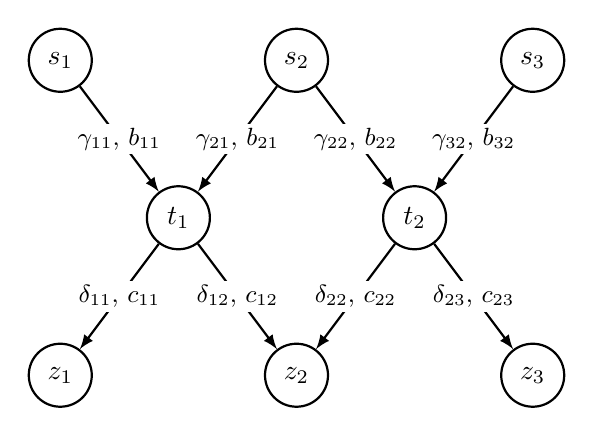
\begin{tikzpicture}[
            nd/.style={circle, draw, minimum size=8mm, inner sep=1pt},
            every edge/.style={draw, -latex, thick},
            lbl/.style={fill=white, inner sep=1.5pt, font=\small},
            thick
        ]
        % Source nodes
        \node[nd] (S1) at (0,4)   {$s_1$};
        \node[nd] (S2) at (3,4)   {$s_2$};
        \node[nd] (S3) at (6,4)   {$s_3$};

        % Treatment plant nodes
        \node[nd] (T1) at (1.5,2) {$t_1$};
        \node[nd] (T2) at (4.5,2) {$t_2$};

        % Demand zone nodes
        \node[nd] (Z1) at (0,0)           {$z_1$};
        \node[nd] (Z2) at (3,0)           {$z_2$};
        \node[nd] (Z3) at (6,0)           {$z_3$};

        % S -> T connections
        \draw (S1) edge node[lbl] {$\gamma_{11},\,b_{11}$} (T1);
        \draw (S2) edge node[lbl] {$\gamma_{21},\,b_{21}$} (T1);
        \draw (S2) edge node[lbl] {$\gamma_{22},\,b_{22}$} (T2);
        \draw (S3) edge node[lbl] {$\gamma_{32},\,b_{32}$} (T2);

        % T -> Z connections
        \draw (T1) edge node[lbl] {$\delta_{11},\,c_{11}$} (Z1);
        \draw (T1) edge node[lbl] {$\delta_{12},\,c_{12}$} (Z2);
        \draw (T2) edge node[lbl] {$\delta_{22},\,c_{22}$} (Z2);
        \draw (T2) edge node[lbl] {$\delta_{23},\,c_{23}$} (Z3);
    \end{tikzpicture}
    \captionof{figure}{One example of the network structure (sources $\to$ treatment plants $\to$ demand zones).
        Each source-plant arc carries $(\gamma_{st}, b_{st})$ and each plant-zone arc carries $(\delta_{tz}, c_{tz})$.
        The formulation is generic over any number of sources, plants, zones and the arcs connecting them; this is only one instance.}
\end{center}

\section{Objective}
Minimise total cost over a single period: the fixed cost of activating each source and plant, the per-ML cost of drawing water, and the per-ML cost of treating it (charged on the volume each plant processes, $\sum_s b_{st}$).

\begin{equation}
    \min \quad
    \underbrace{\sum_{s \in \mathcal{S}} F_s \alpha_s}_{\text{source activation}}
    + \underbrace{\sum_{t \in \mathcal{T}} F_t \beta_t}_{\text{plant activation}}
    + \underbrace{\sum_{s \in \mathcal{S}} C_s a_s}_{\text{drawing water}}
    + \underbrace{\sum_{t \in \mathcal{T}} C_t \sum_{s \in \mathcal{S}} b_{st}}_{\text{plant treatment}}
\end{equation}

\section{Constraints}
\paragraph{Non-negativity.} All continuous flow variables must be non-negative.
\begin{equation}
    a_s, b_{st}, c_{tz} \ge 0, \qquad \forall s \in \mathcal{S}, t \in \mathcal{T}, z \in \mathcal{Z}.
\end{equation}

\paragraph{Demand satisfaction.} The total volume of water sent from all treatment plants to demand zone $z$ via the links $c_{tz}$ must be at least the demand $D_z$ for that zone.
\begin{equation}
    \sum_{t \in \mathcal{T}} c_{tz} \ge D_z, \qquad \forall z \in \mathcal{Z}.
\end{equation}
\paragraph{Source capacity and activation.} Water can only be drawn from a source if it has been activated, and never more than its maximum daily withdrawal.
If the source is inactive ($\alpha_s = 0$) the draw $a_s$ is forced to zero.
If it is active ($\alpha_s = 1$), the draw is capped at $\overline{W}_s$.
\begin{equation}\label{eq:source_capacity}
    a_{s} \le \overline{W}_s\,\alpha_s, \quad \forall s \in \mathcal{S}.
\end{equation}

\paragraph{Plant capacity and activation.} A plant can process water only if it has been activated, up to its throughput capacity.
The total volume arriving from all sources, $\sum_s b_{st}$, is capped at $\overline{V}_t$ and forced to zero when the plant is inactive ($\beta_t = 0$).
\begin{equation}\label{eq:plant_capacity}
    \sum_{s \in \mathcal{S}} b_{st} \le \overline{V}_t \beta_t, \quad \forall t \in \mathcal{T}.
\end{equation}

\paragraph{Plant flow conservation.} The total volume leaving plant $t$ toward all zones via the links $c_{tz}$ equals the total volume entering it from all sources via the links $b_{st}$.
\begin{equation}
    \sum_{z \in \mathcal{Z}} c_{tz} = \sum_{s \in \mathcal{S}} b_{st},
    \quad \forall t \in \mathcal{T}.
\end{equation}

\paragraph{Source flow conservation.} The volume drawn from each source $a_{s}$ must equal the total volume it sends to all plants via the links $b_{st}$.
\begin{equation}
    a_s = \sum_{t \in \mathcal{T}} b_{st} , \quad \forall s \in \mathcal{S}.
\end{equation}

\paragraph{Link capacity.} Each link has a maximum flow and can carry water only if that link is active.
For a source-to-plant link, the flow $b_{st}$ is capped at $\overline{L}_{st}$ and forced to zero unless the link is active ($\gamma_{st} = 1$).
\begin{equation}
    b_{st} \le \overline{L}_{st} \gamma_{st}, \quad \forall s \in \mathcal{S}, t \in \mathcal{T}.
\end{equation}
Similarly, a plant-to-zone link's flow $c_{tz}$ is capped at $\overline{L}_{tz}$ and is zero unless the link is active ($\delta_{tz} = 1$).
\begin{equation}
    c_{tz} \le \overline{L}_{tz} \delta_{tz}, \quad \forall t \in \mathcal{T}, z \in \mathcal{Z}.
\end{equation}

\paragraph{Links require active nodes.} Links can only be active if the corresponding upstream node (source or treatment plant) is active.
This is enforced by ensuring that the binary variables representing the links are less than or equal to the binary variables representing the activation of the sources and plants.
A source-to-plant link requires the source to be active:
\begin{equation}
    \gamma_{st} \le \alpha_s, \quad \forall s \in \mathcal{S}, t \in \mathcal{T}.
\end{equation}
A plant-to-zone link requires the plant to be active:
\begin{equation}
    \delta_{tz} \le \beta_t,  \quad \forall t \in \mathcal{T}, z \in \mathcal{Z}.
\end{equation}
\emph{Optional}: a source-to-plant link could also require the plant to be active,
\begin{equation}
    \gamma_{st} \le \beta_t, \quad \forall s \in \mathcal{S},\, t \in \mathcal{T}.
\end{equation}
This is not explicitly needed, since zero flow to an inactive plant is already guaranteed by the plant capacity constraint \eqref{eq:plant_capacity}.
Suppose plant $t$ is inactive, so $\beta_t = 0$. Then \eqref{eq:plant_capacity} becomes
\begin{equation*}
    \sum_{s \in \mathcal{S}} b_{st} \le \overline{V}_t\,\beta_t = 0,
\end{equation*}
and since every flow is non-negative ($b_{st} \ge 0$), this forces $b_{st} = 0$ for all $s \in \mathcal{S}$.


\paragraph{Water quality.} The water arriving at each plant must stay within the quality limits.
For parameter $p$, $\sum_s Q_{sp} b_{st}$ is the total amount of $p$ entering plant $t$ and $\sum_s b_{st}$ is the total volume, so this keeps the average value of $p$ at the plant between $\underline{Q}_p$ and $\overline{Q}_p$.
\begin{equation}
    \underline{Q}_p \sum_{s \in \mathcal{S}} b_{st}
    \le \sum_{s \in \mathcal{S}} Q_{sp}b_{st}
    \le \overline{Q}_p \sum_{s \in \mathcal{S}} b_{st},
    \quad \forall t \in \mathcal{T},\ \forall p \in \mathcal{P}.
\end{equation}
Each $Q_{sp}$ must be a quantity that blends linearly by volume, so that summing each source's contribution, $\sum_{s \in \mathcal{S}} Q_{sp}\,b_{st}$, correctly represents the blended quality at the plant.

\section{Application to the toy model}
This network model is a generalisation of the Sprint~1 toy model, not a different problem: the toy is the special case with a \emph{single} treatment plant and a \emph{single} demand zone.
With one plant and one zone there is nothing to route: every activated source sends its whole draw to the one plant ($b_{st}=a_s$) and all of it reaches the one zone ($c_{tz}=\sum_s a_s$), so the routing variables $\gamma,\delta,b,c$ are fully determined ($\gamma=\delta=1$, $b_{st}=a_s$, $c_{tz}=\sum_s a_s$) and only the source decisions $\alpha_s,a_s$ remain free.
Formally this is the network model with $\mathcal{T}=\{t\}$, $\mathcal{Z}=\{z\}$, the plant fixed active ($\beta_t=1$) and the routing fixed on ($\gamma_{st}=\delta_{tz}=1$).
Substituting these into the network equations gives the toy model formulation below.

\subsection{Decision variables}
\begin{center}
    \begin{tabular}{@{}llll@{}}
        \toprule
        \textbf{Notation} & \textbf{Domain} & \textbf{Description}           & \textbf{Units} \\
        \midrule
        $\alpha_{s}$      & $\{0,1\}$       & $1$ if source $s$ is activated & ---            \\
        $a_{s}$           & $\ge 0$         & volume drawn from source $s$   & ML/day         \\
        \bottomrule
    \end{tabular}
\end{center}

\subsection{Objective}
Minimise the fixed activation cost of the chosen sources plus the per-ML cost of drawing and treating the water.
The single plant is always on, so its fixed cost $F_t$ is a constant and is dropped.
\begin{equation}
    \min \quad
    \underbrace{\sum_{s \in \mathcal{S}} F_s \alpha_s}_{\text{source activation}}
    + \underbrace{\sum_{s \in \mathcal{S}} C_s a_s}_{\text{drawing water}}
    + \underbrace{C_t\sum_{s \in \mathcal{S}} a_s}_{\text{plant treatment}}
\end{equation}

\subsection{Constraints}
\paragraph{Non-negativity.} The draw from each source must be non-negative.
\begin{equation}
    a_s \ge 0, \qquad \forall s \in \mathcal{S}.
\end{equation}

\paragraph{Demand satisfaction.} The total volume drawn (all of which is delivered to the one zone) meets the zone's demand $D_{z}$.
\begin{equation}
    \sum_{s \in \mathcal{S}} a_s \ge D_{z}.
\end{equation}

\paragraph{Source capacity and activation.} Identical to constraint~\eqref{eq:source_capacity}.

\paragraph{Water quality.} The blend of all drawn sources must lie within each parameter's limits.
\begin{equation}
    \underline{Q}_p \sum_{s \in \mathcal{S}} a_s
    \le \sum_{s \in \mathcal{S}} Q_{sp} a_s
    \le \overline{Q}_p \sum_{s \in \mathcal{S}} a_s,
    \quad \forall p \in \mathcal{P}.
\end{equation}

\begin{center}
    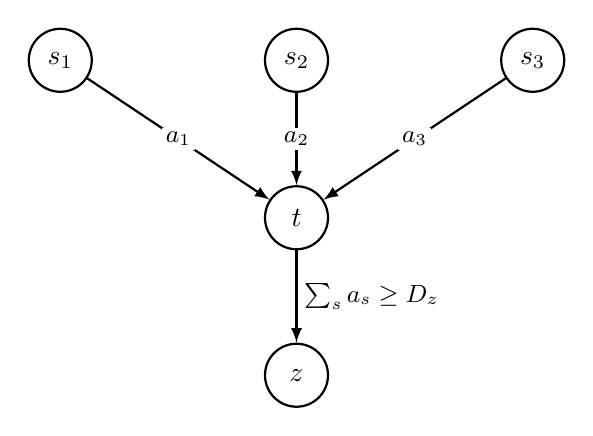
\begin{tikzpicture}[
            nd/.style={circle, draw, minimum size=8mm, inner sep=1pt},
            every edge/.style={draw, -latex, thick},
            lbl/.style={fill=white, inner sep=1.5pt, font=\small},
            thick
        ]
        \node[nd] (s1) at (0,3)   {$s_1$};
        \node[nd] (s2) at (3,3)   {$s_2$};
        \node[nd] (s3) at (6,3)   {$s_3$};
        \node[nd] (t)  at (3,1) {$t$};
        \node[nd] (z)  at (3,-1)   {$z$};
        \draw (s1) edge node[lbl] {$a_1$} (t);
        \draw (s2) edge node[lbl] {$a_2$} (t);
        \draw (s3) edge node[lbl] {$a_3$} (t);
        \draw (t) edge node[lbl, right=1pt] {$\sum_s a_s \ge D_{z}$} (z);
    \end{tikzpicture}
    \captionof{figure}{Toy model: three sources $s_1,s_2,s_3$ feed one plant $t$, which delivers to one zone $z$.
        Routing is fixed, so the delivered blend $\sum_s a_s$ must meet demand $D_z$ and the quality limits.}
\end{center}

\noindent Since this is just the network model with routing fixed, going the other way needs nothing new: free the routing variables and add more sources, plants and zones.
The toy can therefore be built and tested first, then scaled up without reformulating.

\subsection{Additional discrete activation logic}

The base formulation already links source activation to source draw through the
source-capacity constraint. This section records additional discrete activation
logic that can be included where operational assumptions require lower-bound
operation or explicit activation-cost interpretation.

\paragraph{Role of source activation cost.}
The term $\sum_{s \in \mathcal{S}} F_s\alpha_s$ represents the fixed cost incurred
when a water source is activated. This cost applies whenever $\alpha_s=1$,
regardless of the volume drawn from that source. It discourages unnecessary
source activation, particularly where a source contributes only a marginal volume
to the final blend. If reliable fixed activation cost values are not available
during Sprint~1, these values may be set to zero or treated as estimated scenario
parameters.

\paragraph{Optional minimum source-use requirement.}
A minimum source-use requirement may be included to avoid solutions where an
activated source contributes only a negligible volume of water. Let
$\underline{A}_s$ represent the minimum draw required from source $s$ when it is
activated. The constraint is:
\begin{equation}
    a_s \geq \underline{A}_s \alpha_s,
    \quad \forall s \in \mathcal{S}.
\end{equation}

Together with the source-capacity constraint, this defines the operating range:
\begin{equation}
    \underline{A}_s\alpha_s
    \leq
    a_s
    \leq
    \overline{W}_s\alpha_s,
    \quad \forall s \in \mathcal{S}.
\end{equation}

Therefore, if $\alpha_s=0$, source $s$ is inactive and has zero draw. If
$\alpha_s=1$, source $s$ is active and must operate between its minimum-use
requirement and maximum available withdrawal. This constraint is optional in the
Sprint~1 base formulation and may be enabled in scenario analysis if minimum
source-use behaviour is required.

\paragraph{Minimum plant operating flow.}
A treatment plant may be required to operate above a minimum throughput once it
is activated. Let $\underline{V}_t$ represent the minimum operating flow required
for treatment plant $t$. The constraint is:
\begin{equation}
    \sum_{s \in \mathcal{S}} b_{st}
    \geq
    \underline{V}_t\beta_t,
    \quad \forall t \in \mathcal{T}.
\end{equation}

Together with the plant-capacity constraint, this defines the operating range:
\begin{equation}
    \underline{V}_t\beta_t
    \leq
    \sum_{s \in \mathcal{S}} b_{st}
    \leq
    \overline{V}_t\beta_t,
    \quad \forall t \in \mathcal{T}.
\end{equation}

Therefore, if $\beta_t=0$, treatment plant $t$ is inactive and processes no water.
If $\beta_t=1$, treatment plant $t$ is active and must operate between its
minimum operating flow and maximum throughput.

\subsection{Water-quality formulation logic}

This section expands the water-quality constraint in the general formulation by
describing how blended quality is represented for turbidity, alkalinity, and pH.
The aim is to ensure that the selected source flows satisfy the required
water-quality limits while preserving the linear structure of the MILP.

\subsubsection{Purpose of the water-quality formulation}

The water-quality formulation defines how the model represents the quality of
blended water when flows from multiple sources are combined at a treatment plant.
In the general formulation, each source $s$ has a fixed value for each quality
parameter $p$. These values are represented by $Q_{sp}$, where $Q_{sp}$ denotes
the value of quality parameter $p$ in source $s$.

The model uses the source-to-plant flow variables $b_{st}$ to calculate the
blended quality arriving at each treatment plant. For the Sprint~1 model, the
main quality parameters considered are pH, alkalinity, and turbidity. Alkalinity
and turbidity are treated as approximately linear under blending, while pH is
handled by converting raw pH values into hydrogen ion concentration before
optimisation.

\subsubsection{General weighted-average quality logic}

For any quality parameter that blends approximately linearly by volume, the
blended value at treatment plant $t$ can be represented as a volume-weighted
average. The blended value of quality parameter $p$ at plant $t$ is:
\begin{equation}
    Q^{\mathrm{blend}}_{tp}
    =
    \frac{
    \sum_{s \in \mathcal{S}} Q_{sp} b_{st}
    }{
    \sum_{s \in \mathcal{S}} b_{st}
    }.
\end{equation}

Here, $Q_{sp}$ is the quality value of parameter $p$ in source $s$, and $b_{st}$
is the volume of water sent from source $s$ to treatment plant $t$. This
weighted-average structure means that a source has greater influence on the
final blended quality if it contributes a larger volume to the plant.

\subsubsection{Linear quality constraint form}

The blended value of each quality parameter must remain within its allowed lower
and upper limits:
\begin{equation}
    \underline{Q}_p
    \leq
    Q^{\mathrm{blend}}_{tp}
    \leq
    \overline{Q}_p.
\end{equation}

Substituting the weighted-average expression gives:
\begin{equation}
    \underline{Q}_p
    \leq
    \frac{
    \sum_{s \in \mathcal{S}} Q_{sp} b_{st}
    }{
    \sum_{s \in \mathcal{S}} b_{st}
    }
    \leq
    \overline{Q}_p.
\end{equation}

To preserve linearity, the formulation is rearranged by multiplying through by
the total flow into plant $t$:
\begin{equation}
    \underline{Q}_p
    \sum_{s \in \mathcal{S}} b_{st}
    \leq
    \sum_{s \in \mathcal{S}} Q_{sp} b_{st}
    \leq
    \overline{Q}_p
    \sum_{s \in \mathcal{S}} b_{st}.
\end{equation}

This is the load-form quality constraint used in the MILP. It avoids division by
a decision variable and therefore preserves linearity.

\subsubsection{Turbidity formulation}

Turbidity measures the cloudiness of water and is associated with suspended
particles such as sediment, organic matter, algae, clay, or runoff material. In
water-supply modelling, turbidity is important because high turbidity may
increase treatment requirements and affect disinfection performance.

In this formulation, turbidity is treated as approximately linear under blending.
Therefore, for the turbidity parameter, $Q_{sp}$ directly represents the turbidity
value of source $s$:
\begin{equation}
    Q_{sp} = \mathrm{Turbidity}_s.
\end{equation}

The blended turbidity at plant $t$ is:
\begin{equation}
    \mathrm{Turbidity}^{\mathrm{blend}}_{t}
    =
    \frac{
    \sum_{s \in \mathcal{S}} \mathrm{Turbidity}_s b_{st}
    }{
    \sum_{s \in \mathcal{S}} b_{st}
    }.
\end{equation}

If both lower and upper turbidity limits are used, the acceptable range is:
\begin{equation}
    \mathrm{Turbidity}^{\min}
    \leq
    \mathrm{Turbidity}^{\mathrm{blend}}_{t}
    \leq
    \mathrm{Turbidity}^{\max}.
\end{equation}

The corresponding linear constraints are:
\begin{equation}
    \sum_{s \in \mathcal{S}} \mathrm{Turbidity}_s b_{st}
    \geq
    \mathrm{Turbidity}^{\min}
    \sum_{s \in \mathcal{S}} b_{st},
    \quad \forall t \in \mathcal{T},
\end{equation}

\begin{equation}
    \sum_{s \in \mathcal{S}} \mathrm{Turbidity}_s b_{st}
    \leq
    \mathrm{Turbidity}^{\max}
    \sum_{s \in \mathcal{S}} b_{st},
    \quad \forall t \in \mathcal{T}.
\end{equation}

These constraints ensure that the blended turbidity remains within the defined
operating range.

\subsubsection{Alkalinity formulation}

Alkalinity measures the ability of water to neutralise acid. It represents the
buffering capacity of water and is important for pH stability, corrosion control,
treatment performance, remineralisation, and water stability in distribution
systems.

In this formulation, alkalinity is treated as approximately linear under blending.
Therefore, for the alkalinity parameter, $Q_{sp}$ directly represents the
alkalinity value of source $s$:
\begin{equation}
    Q_{sp} = \mathrm{Alkalinity}_s.
\end{equation}

The blended alkalinity at plant $t$ is:
\begin{equation}
    \mathrm{Alkalinity}^{\mathrm{blend}}_{t}
    =
    \frac{
    \sum_{s \in \mathcal{S}} \mathrm{Alkalinity}_s b_{st}
    }{
    \sum_{s \in \mathcal{S}} b_{st}
    }.
\end{equation}

If both lower and upper alkalinity limits are used, the acceptable range is:
\begin{equation}
    \mathrm{Alkalinity}^{\min}
    \leq
    \mathrm{Alkalinity}^{\mathrm{blend}}_{t}
    \leq
    \mathrm{Alkalinity}^{\max}.
\end{equation}

The corresponding linear constraints are:
\begin{equation}
    \sum_{s \in \mathcal{S}} \mathrm{Alkalinity}_s b_{st}
    \geq
    \mathrm{Alkalinity}^{\min}
    \sum_{s \in \mathcal{S}} b_{st},
    \quad \forall t \in \mathcal{T},
\end{equation}

\begin{equation}
    \sum_{s \in \mathcal{S}} \mathrm{Alkalinity}_s b_{st}
    \leq
    \mathrm{Alkalinity}^{\max}
    \sum_{s \in \mathcal{S}} b_{st},
    \quad \forall t \in \mathcal{T}.
\end{equation}

These constraints ensure that the blended alkalinity remains within the required
operating range.

\subsubsection{pH transformation}

pH is handled differently from turbidity and alkalinity because pH is a
logarithmic measure of hydrogen ion concentration. Raw pH values should not be
averaged directly because direct pH averaging can produce a scientifically
misleading blended value.

pH is defined as:
\begin{equation}
    pH = -\log_{10}([H^+]),
\end{equation}
where $[H^+]$ represents hydrogen ion concentration.

To preserve the physical meaning of pH while keeping the MILP formulation
linear, each source pH value is converted into hydrogen ion concentration before
optimisation. For each source $s$, the transformed value is:
\begin{equation}
    H_s = 10^{-pH_s}.
\end{equation}

For the pH quality parameter, $Q_{sp}$ therefore stores the transformed hydrogen
ion concentration $H_s$, not the raw pH value:
\begin{equation}
    Q_{sp} = H_s.
\end{equation}

This allows pH-related blending to be represented using the same linear
load-form structure as the other quality parameters.

\subsubsection{Transformed pH bounds}

The pH limits must also be converted into hydrogen ion concentration limits. If
the acceptable pH range is:
\begin{equation}
    \underline{pH}
    \leq
    pH
    \leq
    \overline{pH},
\end{equation}
then the corresponding hydrogen ion concentration bounds are:
\begin{equation}
    \underline{H} = 10^{-\overline{pH}},
\end{equation}

\begin{equation}
    \overline{H} = 10^{-\underline{pH}}.
\end{equation}

The direction of the bounds changes because pH and hydrogen ion concentration
are inversely related. A higher pH corresponds to a lower hydrogen ion
concentration, while a lower pH corresponds to a higher hydrogen ion
concentration. Therefore, the lower hydrogen ion concentration bound comes from
the upper pH limit, and the upper hydrogen ion concentration bound comes from
the lower pH limit.

\subsubsection{pH constraint in linear form}

After converting source pH values into hydrogen ion concentration, the pH
constraint can be written in the same linear load form as the general quality
constraint. For each treatment plant $t$:
\begin{equation}
    \underline{H}
    \sum_{s \in \mathcal{S}} b_{st}
    \leq
    \sum_{s \in \mathcal{S}} H_s b_{st}
    \leq
    \overline{H}
    \sum_{s \in \mathcal{S}} b_{st},
    \quad \forall t \in \mathcal{T}.
\end{equation}

This constraint ensures that the blended hydrogen ion concentration remains
within the transformed pH bounds. The constraint remains linear because $H_s$,
$\underline{H}$, and $\overline{H}$ are fixed parameters, while $b_{st}$ is the
decision variable.

\subsubsection{Blended pH recovery after optimisation}

The MILP does not directly optimise or report blended pH in raw pH units.
Instead, the optimisation model works with hydrogen ion concentration. After the
solver finds the optimal source-to-plant flows, the blended hydrogen ion
concentration at plant $t$ is calculated as:
\begin{equation}
    H^{\mathrm{blend}}_{t}
    =
    \frac{
    \sum_{s \in \mathcal{S}} H_s b_{st}
    }{
    \sum_{s \in \mathcal{S}} b_{st}
    }.
\end{equation}

The blended pH is then recovered in post-processing as:
\begin{equation}
    pH^{\mathrm{blend}}_{t}
    =
    -\log_{10}
    \left(
    H^{\mathrm{blend}}_{t}
    \right).
\end{equation}

This recovered pH value is not a MILP decision variable. It is a post-solve
reporting value used for validation, interpretation, dashboard display, and
output generation.

\subsubsection{Linearity assumptions for water quality}

The water-quality formulation relies on simplifying assumptions that preserve
linearity in the Sprint~1 MILP. The key assumptions are:
\begin{enumerate}[label=(\roman*)]
    \item water from selected sources is completely mixed before quality is assessed;
    \item the model represents a single time period, so temporal variation in water quality is not modelled;
    \item source quality values are fixed input parameters for the representative period;
    \item alkalinity and turbidity are approximated as volume-weighted linear blends;
    \item raw pH values are not averaged directly; pH is transformed into hydrogen ion concentration before optimisation;
    \item no nonlinear chemical reactions between blended sources are modelled;
    \item chemical dosing does not alter pH, alkalinity, or turbidity in the Sprint~1 toy model;
    \item water quality is checked at the blended output point.
\end{enumerate}

These assumptions allow the water-quality constraints to remain linear and
suitable for inclusion in the MILP formulation.

\end{document}